\documentclass{article}
\usepackage[utf8]{inputenc}
\usepackage[letterpaper,margin=1in]{geometry}
\usepackage{graphicx}
 
\title{\bf{ Lab4: Real-Time Operating Systems} }

\author{Group 2: Shi Su \& Mengjin Yan}
\date{December 2, 2015}
 
\renewcommand*\contentsname{Content}
 
\begin{document}
 
\maketitle
 
\tableofcontents

\newpage

%%%%%%%%%%%
% OVERVIEW
%%%%%%%%%%%

%\section{Overview}
% 
%On the basis of lab2 to implement a small kernel - {\bf Gravel}, adding the IRQ handling and timer driver.\\
%\newline
%\begin{figure}[h]
%\centering
% 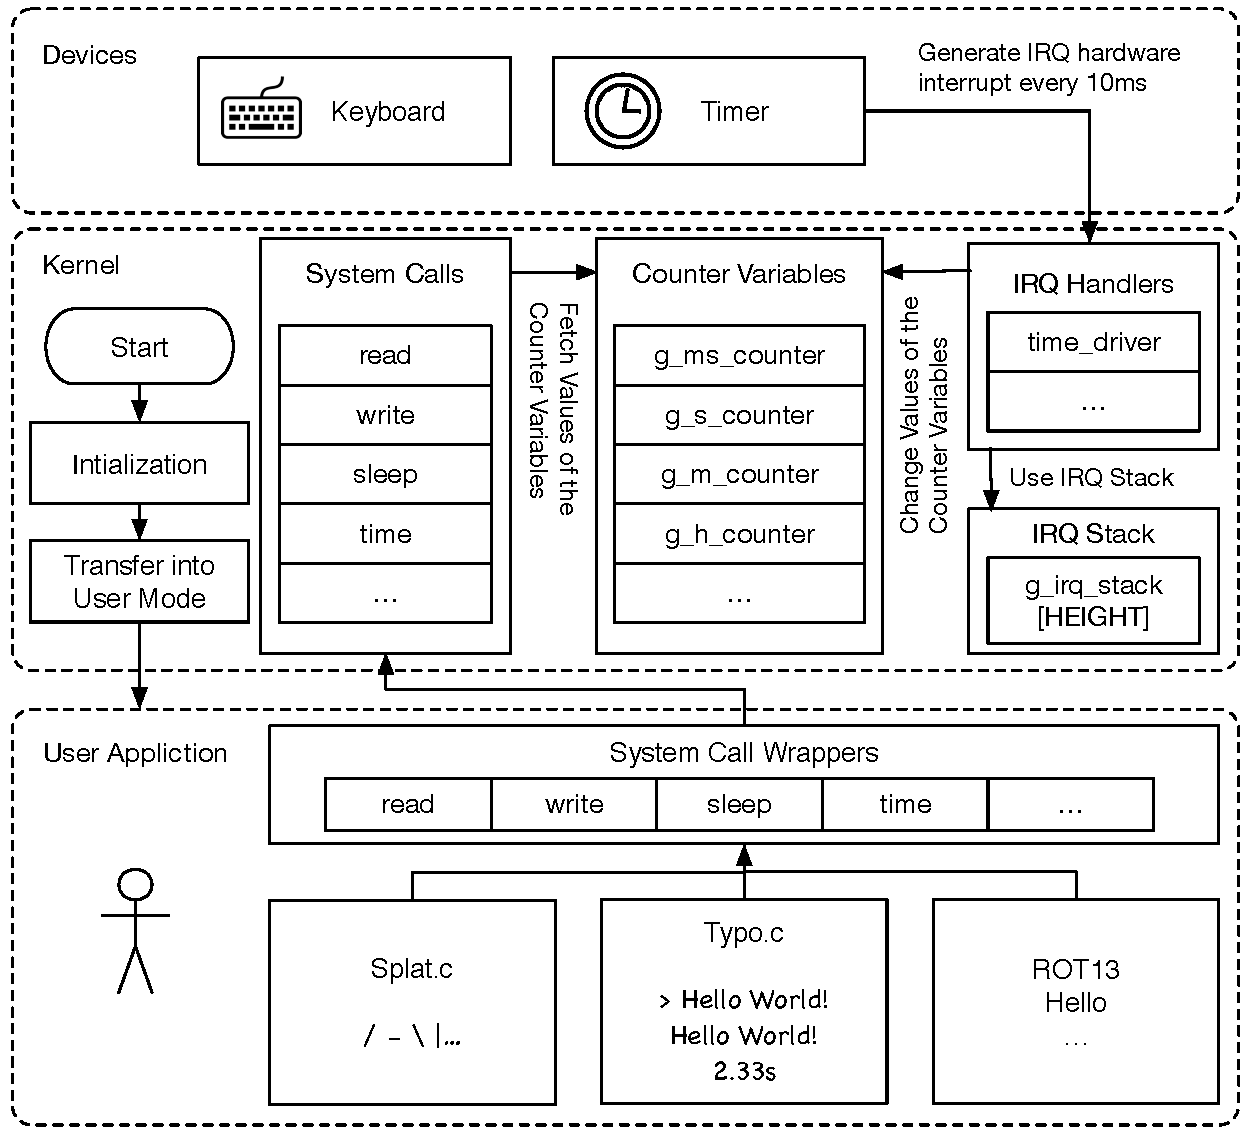
\includegraphics[scale=0.8]{workflow.pdf}\\
% \caption{Modules of Gravel}
% \end{figure}
  
%\newpage

\section{Workflow}
\subsection{Kernel Initiation}
\begin{itemize}
	\setlength{\itemsep}{1pt}
	\setlength{\parskip}{0pt}
	\setlength{\parsep}{0pt}
	\item Store the value of r8 (uboot function table) to global variable {\it global\_data}
	\item Wire in SWI/IRQ handler
	\item Set up IRQ stack\\
		A chuck of memory is allocated for IRQ stack in data section as the global variable array {\it g\_irq\_stack}, we don't need to specified its location explicitly and worry about it will be clobbered by code or stack. Since array grows from lower address to higher address, while the growth direction of stack is opposite. So sp is set to point at the highest address(end) of array {\it g\_irq\_stack}. \\
	\item Initiate interrupt controller\\
		Update ICMR to mask interrupt from all interrupt except OSMR0.\\
		Update ICLR to route interrupt from OSMR0 as IRQ.\\
	\item Initiate Timer
		Set all time counter variables to 0.\\
		Set the value of OSSR to 0\\
		Update OIER to enable the interrupt from OSMR0\\
		Set the value of OSMR0 to 32500, which corresponds to 10ms resolution\\
\end{itemize}

%%%%%%%%%%%
% Task creation
%%%%%%%%%%%
\subsection{Task Creation}
\begin{itemize}
	\setlength{\itemsep}{1pt}
	\setlength{\parskip}{0pt}
	\setlength{\parsep}{0pt}
	\item test
\end{itemize}

%%%%%%%%%%%
% Context Switch
%%%%%%%%%%%
\subsection{Context Switch}
When an IRQ interrupt is generated, the system automatically changes into IQR mode and the interrupt is handled by the IRQ handler which is consist of two parts, irq\_handler.S and c\_irq\_handler.c.\\
In irq\_handler.S:
	 \begin{itemize}
	  \setlength{\itemsep}{1pt}
	  \setlength{\parskip}{0pt}
	  \setlength{\parsep}{0pt}
	\item Store non-banked user/supervisor mode register on stack
	\item Branch into c\_swi\_handler
	\end{itemize}
In c\_irq\_handler.c:
	\begin{itemize}
	  \setlength{\itemsep}{1pt}
	  \setlength{\parskip}{0pt}
	  \setlength{\parsep}{0pt}
	\item Read the value of ICMR to determine which device generated the IRQ 
	\item Branch to corresponding ISR
\end{itemize}

%%%%%%%%%%%
% TIMEDRIVER
%%%%%%%%%%%
\subsubsection{Event Wait}	
As shown in the graph, 4 global variables, {\it g\_ms\_counter}, {\it g\_s\_counter}, {\it g\_m\_counter} and {\it g\_h\_counter}, are maintained as time counter in our system. They records how much time has elapsed since kernel booted up. 
 \begin{itemize}
	  \setlength{\itemsep}{1pt}
	  \setlength{\parskip}{0pt}
	  \setlength{\parsep}{0pt}
	  \item test
\end{itemize}

For every 10ms, an IRQ interrupt is generated from the timer and the system dispatches the interrupt to be handled in the corresponding time\_driver handler. In time\_driver, the corresponding bit in OSSR is cleared and the value of the global variables are updated.\\
\newline
The design of our time counting system successfully separates the register register reading part and the task processing part of the system making it more flexible and convenient when implementing other timer related system calls.
\newline

%%%%%%%%%%%
% New System Calls
%%%%%%%%%%%	
\subsection{New System Calls}
\begin{itemize}
\item{task\_create}\\
	int task\_create(task\_t* tasks, size\_t num\_tasks)\\
	\newline
	{}

\item{mutex\_create}\\
	int mutex\_create(void)\\
	\newline
	{}

\item{mutex\_lock}\\
	int mutex\_lock(int mutex);\\
	\newline
	{}

\item{mutex\_unlock}\\
	int mutex\_unlock(int mutex);\\
	\newline
	{}

\item{event\_wait}\\
	int event\_wait(unsigned int dev);\\
	\newline
	{}
\end{itemize}


	
 
\end{document}